%!TEX root=robocert.tex

The \emph{sequence} notation of \langname{} provides a method of
defining the expected interactions between actors in a robotic model,
optionally with time constraints.  For instance, sequences may specify
how a \robochart{} module uses services offered by a robotic platform.
Sequences resemble UML sequence diagrams.

\chapter{Metamodel}\label{cha:metamodel}
%!TEX root=./robocert.tex

% Metamodel references.
\newcommand{\mnamedelement}{\metaref{NamedElement}}
\newcommand{\mrapackage}{\metaref{RAPackage}}
\newcommand{\mrcpackage}{\metaref{RCPackage}}
\newcommand{\mbasicpackage}{\metaref{BasicPackage}}
\newcommand{\msequence}{\metaref{Sequence}}
\newcommand{\msubsequence}{\metaref{Subsequence}}
\newcommand{\msequencestep}{\metaref{SequenceStep}}
\newcommand{\msequencegap}{\metaref{SequenceGap}}
\newcommand{\msequenceaction}{\metaref{SequenceAction}}
\newcommand{\marrowaction}{\metaref{ArrowAction}}
\newcommand{\mloopaction}{\metaref{LoopAction}}
\newcommand{\mfinalaction}{\metaref{FinalAction}}
\newcommand{\mgapmessageset}{\metaref{GapMessageSet}}
\newcommand{\mextensionalgapmessageset}{\metaref{ExtensionalGapMessageSet}}
\newcommand{\muniversegapmessageset}{\metaref{UniverseGapMessageSet}}
\newcommand{\mmessagespec}{\metaref{MessageSpec}}
\newcommand{\marrowmessagespec}{\metaref{ArrowMessageSpec}}
\newcommand{\mgapmessagespec}{\metaref{GapMessageSpec}}
\newcommand{\mmessagetopic}{\metaref{MessageTopic}}
\newcommand{\meventmessagetopic}{\metaref{EventMessageTopic}}
\newcommand{\moperationmessagetopic}{\metaref{OperationMessageTopic}}
\newcommand{\mcspfragment}{\metaref{CSPFragment}}
\newcommand{\mnamedassertion}{\metaref{NamedAssertion}}
\newcommand{\massertion}{\metaref{Assertion}}
\newcommand{\msequenceassertion}{\metaref{SequenceAssertion}}
\newcommand{\msequenceassertiontype}{\metaref{SequenceAssertionType}}
\newcommand{\mcspmodel}{\metaref{CSPModel}}
\newcommand{\mworld}{\metaref{World}}
\newcommand{\mactor}{\metaref{Actor}}
\newcommand{\mtargetactor}{\metaref{TargetActor}}
\newcommand{\mtarget}{\metaref{Target}}
\newcommand{\mrcmodule}{\metaref{RCModule}}
\newcommand{\mrcmoduletarget}{\metaref{RCModuleTarget}}
\newcommand{\moverridetarget}{\metaref{OverrideTarget}}

This section introduces the abstract syntax (metamodel) of \langname.
It is structured in a top-down manner, with each section introducing a group of
related \langname{} functionality.  Each section contains:

\begin{itemize}
\item
	a class diagram representing the Ecore classes, enumerations, and other
	components that make up the group being discussed;
\item
	descriptions of the components being shown in the class diagram;
\item
	where relevant, examples of the components in terms of the concrete
	syntaxes of \langname.
\end{itemize}

\todo{Once I have a machine on which Sirius works properly, the diagrams should
be replaced with PDFs.  When this happens, the fonts should be aligned to agree
with those in this report.}

\section{Packages}\label{sec:metamodel-top}

\begin{figure}
	\centering
	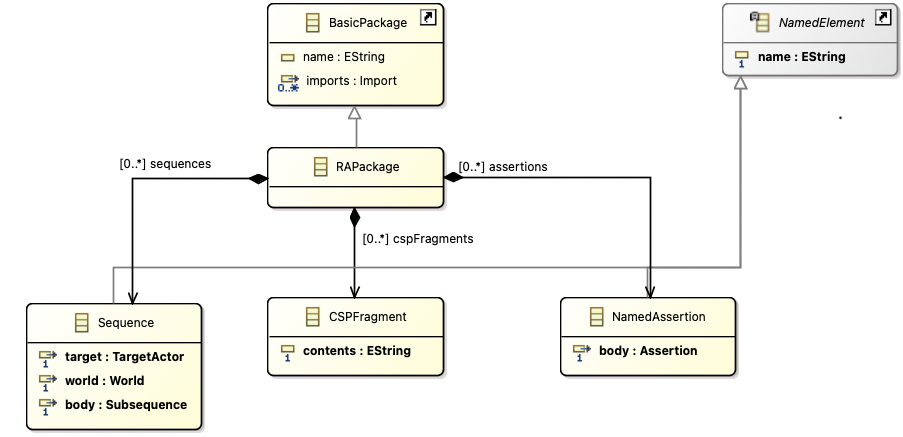
\includegraphics[width=.8\textwidth]{diagrams/top.png}
	\caption{Class diagram for the top of the \langname{} metamodel.}
	\label{fig:metamodel-top}
\end{figure}

\Cref{fig:metamodel-top} is the top-level metamodel diagram for \langname.

Each \langname{} script contains an \mrapackage,\footnote{\mrapackage{} stands
for `RoboStar Assertions package'; we use this name because \mrcpackage{} is
already used for RoboChart packages.}
which is a type of RoboStar \mbasicpackage.
Each \mrapackage{} can contain zero or more of each of these types of content:

\begin{itemize}
\item
	\msequence{}
	(\cref{sec:metamodel-sequences}):
	a sequence diagram;
\item
	\mcspfragment:
	a CSP fragment, currently not bound to a particular process
	\todo{this will change};
\item
	\mnamedassertion{}
	(\cref{sec:metamodel-assertions}):
	a named assertion, currently over sequence diagrams only
	\todo{more types of assertion will appear};
\end{itemize}

\todo{Elements might need to inherit from a common class and be stored in
the same list at some point.}


\section{Sequences, subsequences, and steps}\label{sec:metamodel-sequences}

\begin{figure}
	\centering
	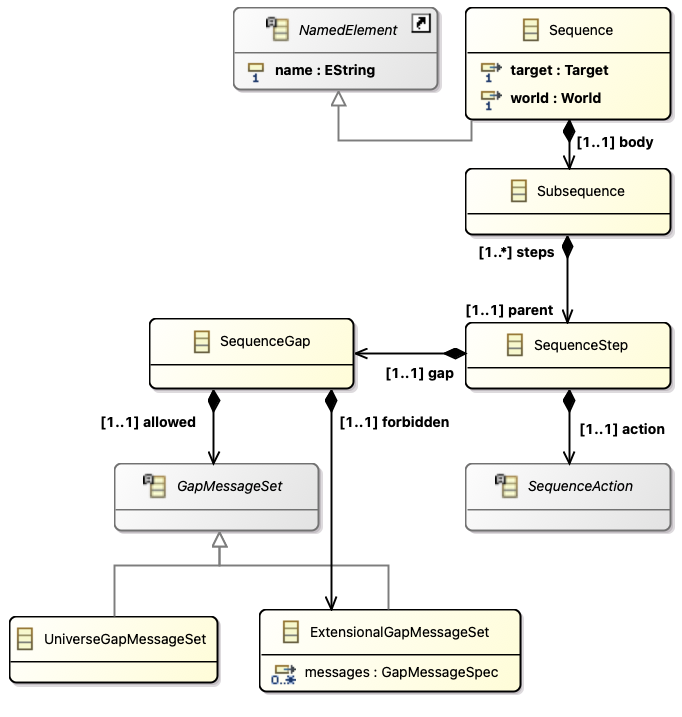
\includegraphics[width=\textwidth]{diagrams/sequences.png}
	\caption{Class diagram for the part of the \langname{} metamodel dealing with sequences.}
	\label{fig:metamodel-sequences}
\end{figure}

\Cref{fig:metamodel-sequences} depicts the part of the metamodel concerning
sequence diagrams.

\subsection{Sequences}

\begin{lstlisting}[style=Example]
sequence Example
  for module ModuleName as M,  // target actor (RoboChart module)
      world             as W   // world actor
{
	anything until end  // subsequence
}
\end{lstlisting}

A \msequence{} represents a single sequence diagram.  It is a \mnamedelement{}
that contains:

\begin{itemize}
\item
	a \msubsequence{} (\cref{ssec:metamodel-sequences-subsequences})
	containing the body of the diagram;
\item
	two \mactor s (\cref{sec:metamodel-actors}):
	a \mtargetactor{} (\cref{ssec:metamodel-actors-target})
	and a \mworld{} (\cref{ssec:metamodel-actors-world}).
\end{itemize}

\subsection{Subsequences}\label{ssec:metamodel-sequences-subsequences}

\begin{lstlisting}[style=Example]
{
	anything until operation O1() from M to W  // step
then
	operation O2() from M to W                 // step
then
	end                                        // step
}
\end{lstlisting}

A \msubsequence{} is a sequential composition of one or more \msequencestep s
(\cref{ssec:metamodel-sequences-steps}).
All \msequence s contain at least one \msubsequence{} at the top level, but
may contain multiple nested \msubsequence s introduced by constructs such as
\mloopaction s.

\subsection{Steps}\label{ssec:metamodel-sequences-steps}

\begin{lstlisting}[style=Example]
anything until             // gap
operation O() from M to W  // action
\end{lstlisting}

A \msequencestep{} is a single step in a \msubsequence.  It consists of a
\msequencegap{} (\cref{ssec:metamodel-sequences-gaps}) and a
\msequenceaction{} (\cref{sec:metamodel-sequences-actions}).

\subsection{Gaps}\label{ssec:metamodel-sequences-gaps}

\begin{lstlisting}[style=Example]
anything
	in     { operation O1() from M to W, operation O2() from M to W }  // allow set
	except { operation O2() from M to W }                              // forbid set

	// a universe set is implied for the allow set if 'in {..}' is omitted
	// an empty extensional set is implied for the forbidden set if 'except {..}' is omitted
until // only permits O1
\end{lstlisting}

A \msequencegap{} represents a condition on any communication\footnote{In PSCs,
this would correspond to \emph{intraMSG}s.} that can happen
\emph{before} a \msequenceaction.  
It contains two \mgapmessageset s: one specifying the messages
\emph{allowed} to pass inside the gap, and another specifying the messages
\emph{forbidden} to pass.\footnote{The \emph{forbidden} set is always an
\mextensionalgapmessageset, as any gap with a universal
\emph{forbidden} set would always be equivalent to one with an empty
\emph{allowed} set.
}

\paragraph{Gap message sets}

A \mgapmessageset{} is an expression of the set of messages allowed or forbidden
inside a \msequencegap.  There are two types of \mgapmessageset:

\begin{itemize}
\item
	a \muniversegapmessageset{} represents the universal set containing 
	all possible messages, and
	captures a lack of specific restriction on
	the \emph{allowed} set of a \msequencegap;
\item	
	an \mextensionalgapmessageset{} is a set (expressed as an unordered list) of
	zero or more \mgapmessagespec s, themselves
	a type of \mmessagespec{} (\cref{sec:metamodel-messages}).
\end{itemize}

There is not yet any meaningful extra data stored in
\mgapmessagespec s that is not present in \mmessagespec s, but this is subject
to change.


\subsection{Actions}\label{sec:metamodel-sequences-actions}

\begin{lstlisting}[style=Example]
operation O1() from M to W  // arrow action

loop L {
	operation O2() from M to W
}  // loop action (taking a subsequence)

end  // final action
\end{lstlisting}

A \msequenceaction{} is an explicit communication or control flow construct in a
\msubsequence.  There are currently three types of action: arrow, loop, and
final actions.

\paragraph{Arrow actions}

An \marrowaction\footnote{The name signifies both that the actions resemble
PSC \emph{arrowMSG} specifications, and also that they correspond to arrows in
the graphical syntax.} specifies one communication between \mactor s which is on
the sequence specified by the diagram.  Each \marrowaction{} wraps one
\marrowmessagespec{} (\cref{sec:metamodel-messages})
containing the specification proper.
\todo{Eventually these will bind arguments.}

\paragraph{Loop actions}

A \mloopaction{} is a \emph{named} infinite loop.  \todo{Breaking and perhaps
other forms of loop are forthcoming.}  Each \mloopaction{} contains one
\msubsequence{} of steps to repeat indefinitely.
\todo{If \mloopaction s could contain zero \msubsequence s, or \msubsequence s
could contain zero \msequencestep s, they could
explicitly capture deadlock, but currently so does \mfinalaction.}

\paragraph{Final actions}

A \mfinalaction{} represents the end of a sequence diagram, corresponding
to a point in time where the sequence target has either terminated or stopped
responding.  It primarily serves to allow a final \msequencegap{} to specify
any permitted communications after the behaviour explicitly specified by the
diagram has occurred.
\todo{Is the termination behaviour correct here?  Are there any useful
parallels between this and a hypothetical empty-bodied loop action?}


\section{Message specifications and topics}\label{sec:metamodel-messages}

\begin{figure}
	\centering
	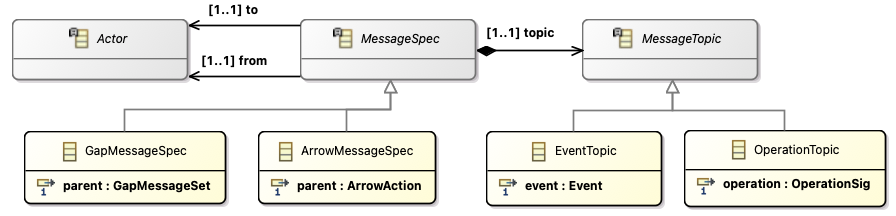
\includegraphics[width=.8\textwidth]{diagrams/messages.png}
	\caption{Class diagram for the part of the \langname{} metamodel dealing with messages.}
	\label{fig:metamodel-messages}
\end{figure}

\Cref{fig:metamodel-messages} depicts the part of the metamodel concerning
message specifications (`specs').

\subsection{Message specifications}

\begin{lstlisting}[style=Example]
operation O1() from M to W  // spec with operation topic, from actor M to actor W
event E        from W to M  // spec with event topic, from actor W to actor M
\end{lstlisting}

A \mmessagespec{} is a specification on the types of communication that can
happen during a gap (a \mgapmessagespec) or arrow (an \marrowmessagespec).\footnote{
This class distinction resembles that in PSCs betweeen intraMSGs and arrowMSGs,
respectively.}  Each \mmessagespec{} contains:

\begin{itemize}
\item
	references to two \mactor s, representing the \emph{to} and \emph{from}
	edges of the communication;
\item
	the \mmessagetopic{} (\cref{ssec:metamodel-messages-topics}) specifying
	the type of communication that the spec is capturing.
\end{itemize}

\subsection{Topics}\label{ssec:metamodel-messages-topics}

A \mmessagetopic{} identifies the specific type of communication in a
\mmessagespec{}.  There are currently two types of topic, corresponding to
RoboChart operations (\moperationmessagetopic) and events (\meventmessagetopic).
Each contains a reference to the signature of the respective construct.
Parameterised operations and events are not yet supported \todo{this will
change soon}.


\section{Actors}\label{sec:metamodel-actors}

\begin{figure}
	\centering
	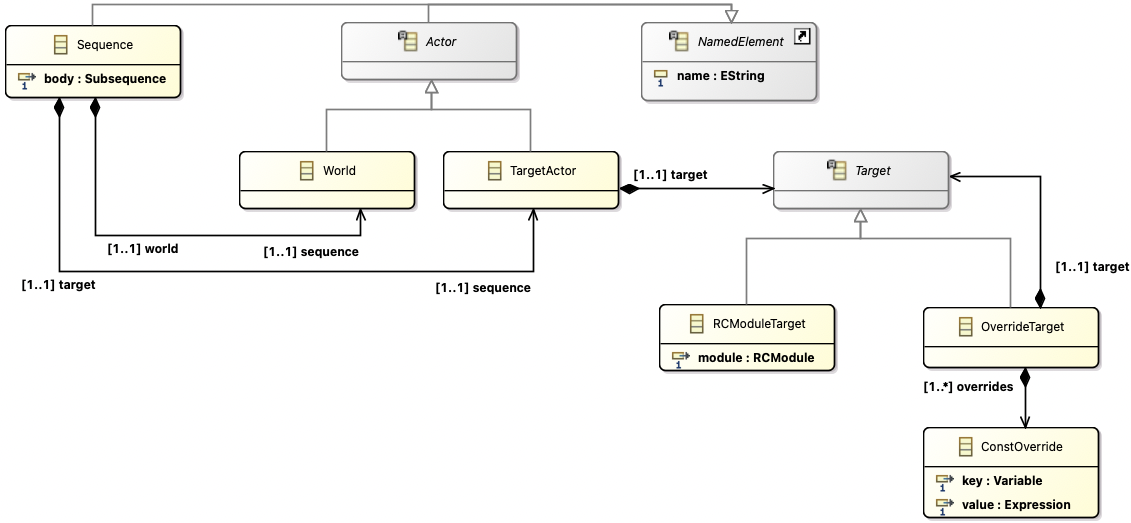
\includegraphics[width=\textwidth]{diagrams/actors.png}
	\caption{Class diagram for the part of the \langname{} metamodel dealing with actors.}
	\label{fig:metamodel-actors}
\end{figure}

\Cref{fig:metamodel-actors} depicts the part of the metamodel concerning
actors.

An \mactor{} is a named participant in a sequence.  The names can be used to
specify the direction of travel in \mmessagespec{}s.
As mentioned in
\cref{sec:metamodel-sequences}, there are always two actors
attached to a sequence: a \mtargetactor{} (\cref{ssec:metamodel-actors-target})
and a \mworld{} (\cref{ssec:metamodel-actors-world}).

\subsection{Targets and target actors}\label{ssec:metamodel-actors-target}

A \mtarget{} is an \emph{anonymous} specification of the part of a robotic
system that serves as the focus for a particular sequence diagram.  There are
presently two types of target, with more to appear later:

\begin{itemize}
\item
	a \mrcmoduletarget{} references a \mrcmodule;
\item
	an \moverridetarget{} wraps another \mtarget, overriding constant
	definitions.
\end{itemize}

A \mtargetactor{} wraps a \mtarget{} with a name, making it suitable as an
\mactor.  The separation between \mtarget{} and \mtargetactor{} allows for
patterns like \moverridetarget{} to exist without introducing unnecessary names.

\subsection{Worlds}\label{ssec:metamodel-actors-world}

A \mworld{} is an \mactor{} that represents the `world' outside a sequence
diagram's target.  \mworld s do not contain any data.

\section{Assertions}\label{sec:metamodel-assertions}

\begin{figure}
	\centering
	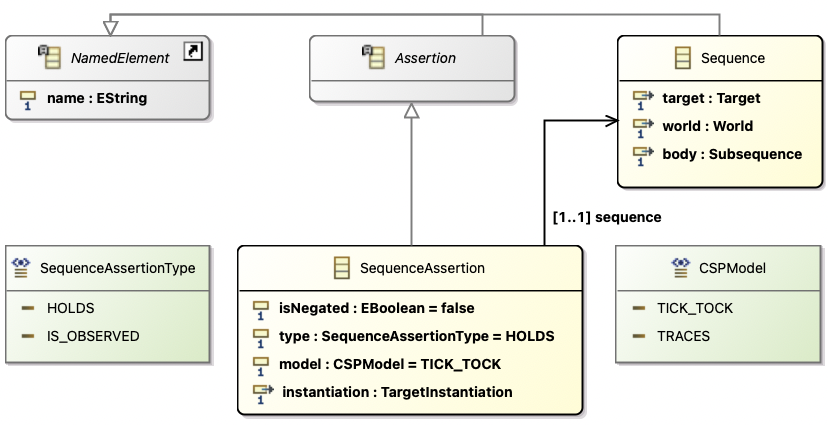
\includegraphics[width=0.7\textwidth]{diagrams/assertions.png}
	\caption{Class diagram for the part of the \langname{} metamodel dealing with assertions.}
	\label{fig:metamodel-assertions}
\end{figure}

\Cref{fig:metamodel-assertions} depicts the part of the metamodel concerning
assertions.

An \massertion{} is an \emph{anonymous} assertion statement.  Currently, there is
only one type of assertion: a \msequenceassertion{}.  \todo{This will change
when merging with the existing language, if not sooner.}

A \msequenceassertion{} is an assertion about a particular \msequence{} with
respect to a particular \mtarget.  By default, the \mtarget{} is that of the
\msequence{}. \todo{This isn't yet explicit in the metamodel.}  Specifying a
custom \mtarget{} as part of the assertion instead makes the assertion refer
to that target.

The specific sequence assertion type comes from the \msequenceassertiontype:
either `sequence holds on target' (refinement), or `sequence is observed on
target' (reverse refinement).  The assertion can be negated.  The choice of
\mcspmodel{} affects how the assertion is checked with CSP tools such as FDR
\todo{the models are incorrect in respect to timed assertions; I haven't yet
decided the best approach to allow the appropriate models in both timed and
untimed modes.  Currently, everything is untimed, and this too will change.}

A \mnamedassertion{} binds an \massertion{} to a name.


\chapter{Textual syntax}\label{cha:seq-textual}
This section describes the textual syntax of \langname{} sequence
diagrams.  This syntax primarily uses controlled English, with
some use of braces and symbols to impose further structure.

\todo{TODO}

%%% Local Variables:
%%% mode: latex
%%% TeX-master: "../robocert"
%%% End:


\chapter{Graphical syntax}\label{cha:seq-graphical}
This section describes the graphical syntax of \langname.

\todo{TODO}

\section{Principles}

\todo{These need work.}

\begin{itemize}
\item Where possible, we draw graphical cues from existing notations.
  This simplifies the uptake of the language for practitioners
  familiar with those notations.  Generally, cues for features come
  from whichever language is identified as the main inspiration in
  \cref{sec:metamodel-features}.
\item Where graphical elements attach to one side of a sequence diagram,
  we choose the side that is most relevant to that element.  For instance:
  \begin{itemize}
  \item \msequencegap s on \marrowaction s attach to whichever
    side is the source of the arrow, to emphasise that the gap modifies
    the act of \emph{sending} the message \todo{I'm not sure this is convincing};
  \item \msequencegap s on \mfinalaction s attach to the \mtarget{} end,
    since the \mfinalaction{} is similar to a message from the \mtarget{} to
    the \mworld{} specifying the \mtarget{} is finished.
  \end{itemize}
\end{itemize}

%%% Local Variables:
%%% mode: latex
%%% TeX-master: "robocert"
%%% End:

\chapter{Comparison with existing notations}\label{cha:seq-comparison}
%!TEX root=../robocert.tex
This chapter compares the \langname{} semantics against formal semantics
proposed for similar efforts.  For instance, we compare the semantics of
sequences against those of UML sequence diagrams and derived notations.

\section{Review by notation}\label{sec:semantics-comparison-review}
% !TEX root=../../robocert.tex

This section reviews each of the above notations in turn, comparing
\langname{} sequences to each.  (We review semantics
later on, in \cref{sec:semantics-comparison-review-seq}.)

\subsection{UML 2.5.1 sequence diagrams}

UML sequence diagrams are a well-understood, standardised notation for
specifying properties over sequences of multi-actor interactions.  As such, they
are an obvious first point of inspiration and comparison.  We track the most
recent standard at time of writing (UML 2.5.1).

\paragraph{Control flow features}
UML 2.5.1 contains generalised notions of selection (the `alt' combined fragment),
optionality (`opt'), iteration (`loop', with support for unbounded and many
forms of numerically bounded loops), parallel composition (`par'), weak ordering
(by default or with `seq'), strict ordering (`strict'), and the inclusion of
other sequences into a sequence (`ref'), amongst others.

\paragraph{Timing features}
UML 2.5.1 dedicates section 8.4 to basic notions of time.  This
support comes in \emph{time} and \emph{duration} (difference between two points
in time) primitives, further divided into \emph{observations} (inspecting the
moment in time when, or duration since, some event occurred) as well as
\emph{constraints} (specifying the time or duration of one or more events).
Constraints can to refer to observations, allowing complex situations such as
`this set of events should happen in at most three times the duration that
this other set of events happened in'.  Duration constraints take the
form of intervals between minimum and maximum permitted duration.

At the moment, our \mdeadlinestep{} construct resembles a UML duration
constraint with minimum duration \(0\).  We do not support observations.

\paragraph{Probabilistic features}
None of which we are aware, outside of extensions to STAIRS (see below).

\subsection{MARTE}

MARTE is a UML profile for real-time systems.

\paragraph{Control flow features}
As UML.

\paragraph{Timing features}
MARTE 1.2 dedicates section 9 to three classes of time abstraction:
casual, synchronous (discrete, clocked), and physical (real-time).  Our work
only covers discrete-time
situations.

MARTE has rich support, using its \emph{Value Specification Language}, for
constraining the durations of message-passing as well as parts of lifelines,
allowing constraints at both local
and global scope\todo{Getting this from Ebeid et al, but I'm not sure that's the
right citation}.  We do not yet support this level of richness.

\paragraph{Probabilistic features}
None of which we are aware.

\subsection{STAIRS}

STAIRS is an approach for incremental, refinement-based development of
UML sequence diagrams capturing existing systems.  We consider it
because it adds features that are not available in UML2, but useful when
following such development processes.

The STAIRS sense of refinement primarily involves the growth of
specifications from sequence diagrams.  It encompasses
notions of \emph{supplementing}, \emph{narrowing}, and
\emph{detailing} sequence diagrams to achieve a more
comprehensive specification.

\paragraph{Control flow features}

STAIRS adds to UML 
a distinction between \emph{potential} behaviour (nondeterminism
in the specification) and \emph{mandatory} behaviour (things the
specification \emph{must} offer the environment)---for example,
an \texttt{xalt} operator that states that all of the choices
must be offered to the environment (unlike \texttt{alt}) which
is cast as an underspecification.
This is
useful from a stepwise refinement perspective, and also
parallels the distinction in CSP between
\(\intchoice\) and \(\extchoice\).

\paragraph{Timed features}
Timed STAIRS is comparable to UML in this regard.

\paragraph{Probabilistic features}
Probabilistic STAIRS adds a
\texttt{palt} operator where choices have associated probability
sets.

\subsection{Message Sequence Chart (MSC)}

ITU message sequence charts~\cite{Harel03-MSC} are a form of sequence diagram
that serves as a precursor to many of the other notations
discussed here, including version 2 and onward of UML.

\paragraph{High-level MSC}

While MSCs do not directly support concepts such as choice and iteration
(to the best of our knowledge), there are extensions that do.  One extension
of interest is \emph{high-level} message sequence charts, which are finite state
automata whose states are labelled with message sequence charts.  This concept
leads to high levels of expressivity (while still being possible to capture in
terms of a semantics), but means that the overall diagram is no longer a single
chart.

\paragraph{Control flow features}
MSCs have very little inherent control flow, being primarily just
sequences of messages (possibly with timing constraints)

\paragraph{Timing features}
As of MSC-96, MSCs had time constraints in the form of both interval
constraints and timer/timeout pairs.

\paragraph{Probabilistic features}
There are no innate probabilistic features in MSCs.

\textcite{Krivanek09-PMSC}, in his bachelor dissertation, proposes a
probabilistic extension of MSC that adds probability in two
ways: first, in attaching probability \emph{distributions} to
durations of messages; second, in the transitions of a HMSC.  While
this proposal seems not to have been realised, the same
dissertation mentions stochastic message sequence charts (which
achieve the first point) and translation into deterministic and
stochastic Petri nets (which achieve part of the second point).

\subsection{Live Sequence Chart (LSC)}

LSC~\cite{lsc} is a
variant of MSC addressing a perceived lack of expressivity.
LSC has several features that are of interest from a \langname{} perspective:

\begin{itemize}
\item visual distinction between mandatory and provisional (or `hot'
  and `cold') elements, the metaphor being that `hot' areas of the
  chart are too hot to stay in for any period of time;
\item conditions that may also be `hot' (abort the
  chart) or `cold' (exit control flow);
\item charts directly carrying universal or existential semantics (with the
  goal of allowing a transition from use-case analysis to specifications);
\item time constraints using the setting, resetting, and comparing of timers;
\item an explicit environment lifeline, to which constraints on the
  environment can be added;
\item `pre-charts', charts that specify the previous communication
  that needs to occur for the main chart to become live.
\end{itemize}

A theme in the LSC development is progressive enhancement: charts move
from existential to universal as more use-case information appears,
and parts of charts move from cold to hot as more knowledge about
liveness appears.

While the \emph{assert} and \emph{negate} aspects of UML2 sequence diagrams
are similar to LSC temperature, \textcite{Harel08-ModalSD} argue
that temperature is not compatible with the trace-set-pair semantics typically
given to UML.  They instead propose a profile of UML implementing the
dichotomy as a modality, with a formal semantics in terms of B\"uchi automata.

LSC variants are still in use as of 2021.  For instance,
\textcite{Chai21-PMLSC} report on a use of `parameterized modal
live sequence charts' to verify train control systems at run-time.

\paragraph{Control flow features}

While the original formulation of LSC~\cite{lsc} seems not to have any
control flow features other than those available in ordinary MSC,
\textcite{Harel03-MSC} attribute both bounded/unbounded loops and some
form of alternative blocks to LSC.

\paragraph{Timing features}
While the original formulation of LSC~\cite{lsc} had no timing
features, later iterations do.
\textcite{Harel03-MSC} propose an encoding of timing constraints in
LSC using a straightforward extension of their existing notation for
constraints, using an implicit timer variable.  A later account by
\textcite{Brill04-LSCintro} suggests a different encoding of
constraints closer to MSC-96.

\paragraph{Probabilistic features}
\textcite{Kai14-PLSC} propose an extension to LSC to capture
probabilistic choice (`probabilistic switch'), as well as
probabilities over aspects of the sending, transmitting, and receiving
of events.

\subsection{Property Sequence Chart (PSC)}

PSC extends a subset of UML2 sequence diagrams (with inspiration from
Message Sequence Charts) to provide a
user-friendly layer atop linear temporal logic.  This is
similar to the general concept of \langname{} sequences with respect to \tockcsp{}
etc., though without the
specific focus on properties of \robochart{} models.
Extensions add timing (TPSC~\cite{tpsc}) and
probabilistic (PTPSC~\cite{ptpsc}) features.

A key difference between PSC and our work is that we are
targeting \todo{for now} properties easily expressed as refinement questions
(and so as artefacts such as CSP processes), whereas PSC targets properties
expressible as linear temporal logic.  We do not yet target LTL,
either directly or by any work that encodes fragments of LTL into
CSP~\cite{fdrspin,Lowe08-CommunicatingProcessSpecification}.

\paragraph{Control flow features}
PSC is considerably streamlined from UML and HMSC, with a small set of operators: strict
ordering; looping; alternative; parallel composition; messages; and constraints.
UML assertion and negation blocks do not exist, in favour of message modalities.

\paragraph{Timing features}
TPSC and PTPSC have clock constraints.  These complement the existing PSC constraint system
(which loosely corresponds to our concept of gaps), adding the ability to
specify that the occurrence of certain messages satisfies an inequality against
a named and resettable clock.

\paragraph{Probabilistic features}
PTPSC divides sequences into two sections: a LSC-style pre-chart where no messages can be required,
and a main chart with a probability inequality.  This gives a coarse-grained notion of `if we see
this behaviour, then this behaviour occurs with a certain probability'.

\subsection{Non-graphical languages}

We also consider the following languages and projects that, while not
graphical, are important in the area of property specification.

\paragraph{Property Specification Patterns (PSP)}

This long-running work by Dwyer et al. forms a repository of
structured patterns for structuring the specification of temporal
properties for concurrent and reactive systems.  These patterns have names,
known modes of composition, and example mappings into temporal logics.

\paragraph{Autili, Grunske, Lumpe, Pelliccione, and Tang (AGLPT)}

This work proposes a structured English grammar covering many of the Property
Specification Patterns.  The grammar provides for timing and probabilistic
features.

\subsection{Common themes and differences}

Summarising the above, we can find the following common
themes and differences in existing sequence
diagram languages:

\paragraph{Themes}

\begin{itemize}
\item
  Two axes, usually discrete:
  \begin{itemize}
  \item
    one distinguishing between participants in an interaction;
  \item
    another providing some form of time ordering;
  \end{itemize}
\item
  Message passing across the participant axis as the main expression of
  interaction;
\item
  Control flow manipulated by blocks 
  spanning both axes;
\item
  Often, \emph{some} notion of mandatory and provisional
  (sometimes also forbidden) behaviour;
\item
  Time and duration constraints, whether natively or through extension;
\item
  Support for probabilities, whether natively or through extension.
\end{itemize}

\paragraph{Differences}

\begin{itemize}
\item The target semantics (see
  \cref{sec:semantics-comparison-review});
\item Whether time constraints are available and, if so, how they work
  (for instance, clocks versus duration spans);
\item Whether probabilistic operators are available and, if so, how
  they work and their granularity;
\item The specifics of event ordering, especially with respect to
  communications happening on vertically disjoint lifelines but
  horizontally similar time-slices;
\item The precise form of the mandatory and provisional behaviour
  specification; for instance, temperature in LSC vs message types in
  PSC vs control blocks.
\end{itemize}

%%% Local Variables:
%%% mode: latex
%%% TeX-master: "../../robocert"
%%% End:

\section{Analysis of decision points}\label{sec:semantics-comparison-review}
%!TEX root=../../robocert.tex

\todo{Non-sequence languages}

\subsection{Sequences}

The survey by Micskei and Waeselynck gives identifies many decision points that
distinguish derivations of semantics for UML and UML-style sequence diagram
languages, with a worked example in the form of the
UML2-derived sequence diagram language \emph{TERMOS}.
We can follow a similar process for \langname{} sequences, as follows:

\begin{description}
\item[Representing events]
  \langname{} represents events as (action, sender, receiver, message name)
  tuples at a metamodel level (see \cref{sec:metamodel-messages}),
  though for 2-actor sequences the sender and
  receiver are implicit in the direction, and in the \tockcsp{} semantics a
  notion of typed channels also renders some aspects of the encoding implicit.
  There is no way to distinguish, given two identical sends occurring at the
  same instant in time, which was responsible for which corresponding receive;
  we do not think that this distinction is important for our use case
  \todo{is it?}
\item[Categorising traces]
  \langname{} is a verification language and (contravening UML2)
  uses a two-category approach: valid/other or invalid/other, depending on the
  \metafeature{isNegated} flag on the \massertion.
  As the main \langname{} semantics is \tockcsp, we use a
  refinement-style categorisation where a sequence denotes an
  expected set of traces (or stable failures, and so on) that must be a superset
  of those calculated from the target.
\item[Complete or partial traces]
  \langname{} sequences (contravening UML2) are \emph{partial} with, by default,
  any suffix permitted.  Prefixes may be permitted by using gaps at the start of
  the sequence.  This difference reflects the underlying trace model of \tockcsp.
  \todo{Ana mentioned a good reason for why we might want this semantics that
  isn't just `CSP does it', but I can't remember precisely what it was.
  Compositionality?}
\item[Combining fragments]
  \langname{} sequences (contravening UML2) currently synchronise on entering
  their equivalent of combined fragments.  \todo{This doesn't actually matter
  yet for 2-actor sequences.}
\item[Processing the diagram]
  \langname{} sequences tend to have a compositional semantics whereby metamodel
  concepts translate bottom-up into fragments of
  the object language, with combined fragments translating into the relevant
  operators,
  and additional superstructure such as memory processes and parameterisations
  being added as needed.
\item[Underlying formalism: Approach]
  The \langname{} semantics maps each sequence to a representation in another
  language, to which we delegate the choice of approach.
  In at least the example of \tockcsp, the end result is a calculation of the
  set of all possible traces (or similar denotation), which corresponds at
  least partially to UML2.
\item[Underlying formalism: Concurrency]
  \langname{} sequences have an interleaving semantics, in accordance with
  both UML2 and \tockcsp.
\item[Handling choices]
  Not set yet
  \todo{I suspect this will create a global time point for the choice.}
\item[Interpretation of a false guard]
  Not set yet.
  \todo{I suspect this will act as in CSP eg pulling the alternative down to
  \(\Stop\).}
\item[Who evaluates a guard]
  Not set yet.
  \todo{I suspect this would be the memory process, which would suggest a
  global evaluation.}
\item[Formal and actual Gates]
  These do not exist in \langname{} sequences.
\item[Interpretation of \texttt{neg(S)}]
  These do not exist in \langname{} sequences.
\item[Ignore/consider]
  These do not exist in \langname{} sequences.
\item[Conformance-related operators in complex diagrams]
  \langname{} sequences have no conformance-related operators at the diagram
  level; sequences always represent a set of possible traces (or similar
  denotation) to be compared against those observable from a model.
\item[Traces being both valid and invalid]
  Theoretically, all traces are either allowed or disallowed by the diagram,
  with the lack of features for characterising traces within the diagram itself
  serving as a restriction to enforce this.  It may not
  be decidable to verify that all traces exhibitable by a model are allowed by
  the diagram (or that one trace disallowed by the diagram is never observable
  in the model).
\end{description}


%%% Local Variables:
%%% mode: latex
%%% TeX-master: "robocert"
%%% End:
